\section{中断点亮小灯}
示例程序int实现功能为中断控制控制LED灯亮,此处分析int程序
\subsection{原理分析}
利用S3C2440手册,分析解读中断初始化程序。S3C2440A 中的中断控制器接受来自 60 个中断源的请求。
提供这些中断源的是内部外设,如 DMA 控制器、UART、IIC 等等。在这些中断源中,
UARTn、AC97 和 EINTn 中断对于中断控制器而言是“或”关系。
当从内部外设和外部中断请求引脚收到多个中断请求时,中断控制器在仲裁步骤后请求
 ARM920T 内核的 FIQ或 IRQ。仲裁步骤由硬件优先级逻辑决定并且写入结果到帮助用户
 通告是各种中断源中的哪个中断发生了的中断挂起寄存器中。\\
 \\
 控制流程图如下:\\
\begin{figure}[htbp]
  \centering
  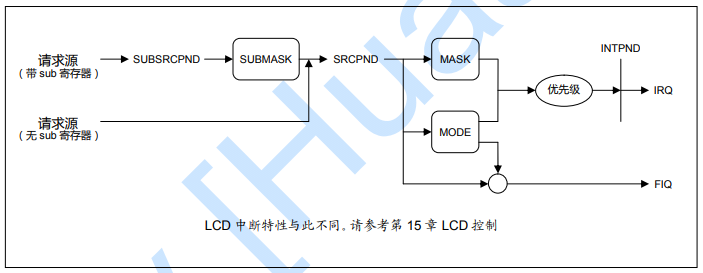
\includegraphics[width=1\textwidth]{int1.png}
  \caption{中断控制流程图}
\end{figure}
\\
1. 先收集到SRCPND\\
2. 用INTMOD判断是否为FIQ\\
3. 判断完后进入屏蔽环节INTMSK进行筛选\\
4. PRIORITY进行优先级划分\\
5. 划分结果存储在INTOFFSET\\
\\
\\
\\
\\
\\
\\
\\
原理图如下:\\
\begin{figure}[htbp]
  \centering
  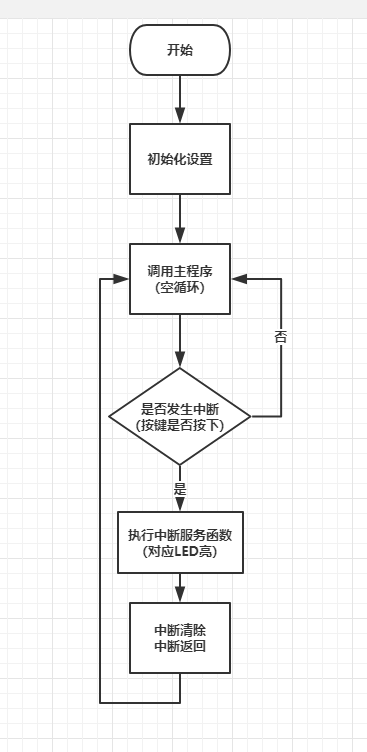
\includegraphics[width=0.3\textwidth]{sch1.png}
  \caption{中断点亮小灯原理图}
\end{figure}

\subsection{调试过程}
\subsubsection{中断初始化程序分析}
head.s程序:\\
功能:初始化,设置中断模式、管理模式的栈,设置好中断处理函数。\\
\lstset{language=bash}
\begin{lstlisting}{中断初始化程序}
  Reset:                  
  ldr sp, =4096           
  bl  disable_watch_dog   
  msr cpsr_c, #0xd2       @ 进入中断模式
  ldr sp, =3072           @ 设置中断模式栈指针

  msr cpsr_c, #0xd3       @ 进入管理模式

  bl  init_led            @ 初始化LED的GPIO管脚
  bl  init_irq            @ 调用中断初始化函数,在init.c中
  msr cpsr_c, #0x5f       @ 设置I-bit=0,开IRQ中断
  
  ldr lr, =halt_loop      @ 设置返回地址
  ldr pc, =main           @ 调用main函数
halt_loop:
  b   halt_loop
\end{lstlisting}
此段代码为中断初始化的核心,设置了中断开启的模式,并调用了各个初始化函数,如\lstinline{init_led}
和\lstinline{init_irq}

\lstset{language=bash}
\begin{lstlisting}{中断跳转程序}
HandleIRQ:
    sub lr, lr, #4                  @ 计算返回地址
    stmdb   sp!,    { r0-r12,lr }   @ 保存使用到的寄存器
                                    @ 注意,此时的sp是中断模式的sp
                                    @ 初始值是上面设置的3072
    
    ldr lr, =int_return             @ 设置调用ISR即EINT_Handle函数后的返回地址  
    ldr pc, =EINT_Handle            @ 调用中断服务函数,在interrupt.c中
\end{lstlisting}
此处为中断跳转程序,当出现特定中断时会跳转到这里,然后按照这里的指示跳转到中断服务函数,这里是跳转到
\lstinline{EINT_Handle}内。

\subsubsection{中断寄存器分析}
打开\lstinline{s3c24xx.h},这里使用到的interrupt registes,我们可以看到
\lstset{language=C}

\begin{lstlisting}{中断寄存器}
#define SRCPND              (*(volatile unsigned long *)0x4A000000)
#define INTMOD              (*(volatile unsigned long *)0x4A000004)
#define INTMSK              (*(volatile unsigned long *)0x4A000008)
#define PRIORITY            (*(volatile unsigned long *)0x4A00000c)
#define INTPND              (*(volatile unsigned long *)0x4A000010)
#define INTOFFSET           (*(volatile unsigned long *)0x4A000014)
#define SUBSRCPND           (*(volatile unsigned long *)0x4A000018)
#define INTSUBMSK           (*(volatile unsigned long *)0x4A00001c)
\end{lstlisting}
这里使用了大量中断相关寄存器。其中
SRCPND:当一个中断发生后,那么相应的位会被置1,
表示一个或一类中断发生了。\\
INTMOD:当INTMOD中某位被设置为1时,它对应的中断被设为FIQ,
CPU将进入快速中断模式。\\
INTMSK:32位,用来屏蔽SRCPND寄存器所标识的中断。
但只能屏蔽IRQ中断,不能屏蔽FIQ中断。\\
PRIORITY:用于设置IRQ中断的优先级。\\
INTPND:中断优先级仲裁器选出优先级最高中断后,
这个中断在INTPND寄存器中的相应位被置1,随后,CPU进入中断模式处理它。
同一时间内,此寄存器只有一位被置1。\\
INTOFFSET:用来表示INTPND寄存器中哪位被置1了
,即记录INTPND中位[x]为1的位x的值。清除INTPND、SRCPND时自动清除。\\
SUBSRCPND:次级源挂起寄存器,当一个中断发生后,
那么相应的位会被置1,表示一个中断发生了。\\
INTSUBMSK:中断次级屏蔽寄存器,此寄存器有 11 位,
其每一位都与一个中断源相联系。如果某个指定位被设置为 1,
则相应中断源的中断请求不会被 CPU 所服务(请注意即使在这种情况中
,SRCPND 寄存器的相应位也设置为 1)。如果屏蔽位为0,则可以服务
中断请求。\\
\subsubsection{中断寄存器配置}
打开\lstinline{init.c},这里对中断寄存器配置,我们可以看到
\lstset{language=C}
\begin{lstlisting}{中断寄存器配置}
  void init_irq( )
  {
      // S2,S3对应的2根引脚设为中断引脚 EINT0,ENT2
      GPFCON &= ~(GPF0_msk | GPF2_msk);
      GPFCON |= GPF0_eint | GPF2_eint;
  
      // S4对应的引脚设为中断引脚EINT11
      GPGCON &= ~GPG3_msk;
      GPGCON |= GPG3_eint;
      
      // 对于EINT11,需要在EINTMASK寄存器中使能它
      EINTMASK &= ~(1<<11);
          
      /*
       * 设定优先级:
       * ARB_SEL0 = 00b, ARB_MODE0 = 0: REQ1 > REQ3,即EINT0 > EINT2
       * 仲裁器1、6无需设置
       * 最终:
       * EINT0 > EINT2 > EINT11即K2 > K3 > K4
       */
      PRIORITY = (PRIORITY & ((~0x01) | (0x3<<7))) | (0x0 << 7) ;
  
      // EINT0、EINT2、EINT8_23使能
      INTMSK   &= (~(1<<0)) & (~(1<<2)) & (~(1<<5));
  }
\end{lstlisting}
2440的外部中断引脚EINT与通用IO引脚F和G复用,要想使用中断功能,
就要把相应的引脚配置成中断模式,如我们想把端口F0设置成外部中断,
而其他引脚功能不变,则\lstinline{GPFCON=(GPFCON & ~0x3) | 0x2}。 \\
\\
配置完引脚后,还需要配置具体的中断功能。我们要打开某一中断的屏蔽,
这样才能响应该中断,相对应的寄存器为INTMSK;还要设置外部中断的触发方式,
如低电平、高电平、上升沿、下降沿等,相对应的寄存器为EXTINTn。
另外由于EINT4到EINT7共用一个中断向量,EINT8到EINT23也共用一个中断向量,
而INTMSK只负责总的中断向量的屏蔽,
要具体打开某一具体的中断屏蔽,还需要设置EINTMASK。\\

还有一些其他的配置,如当需要用到快速中断时,要使用INTMOD,当需要配置中断优先级时,要使用PRIORITY等。
优先级如下:\\
\\
\\
\begin{figure}[htbp]
  \centering
  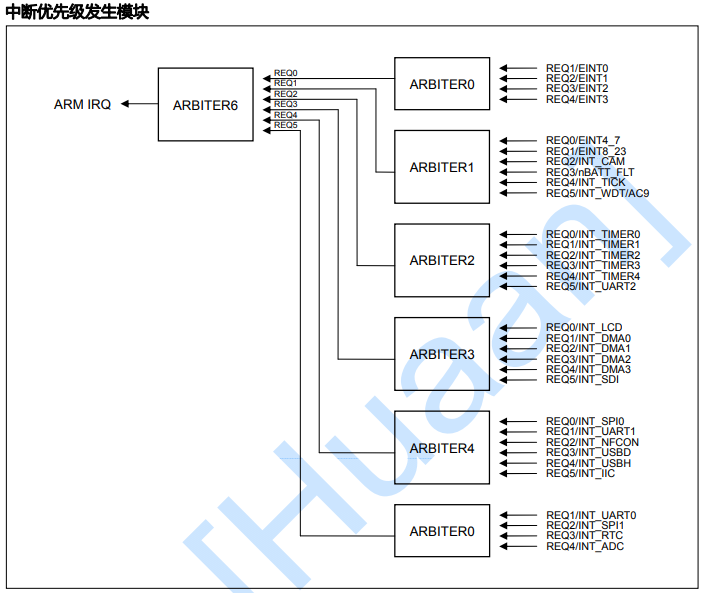
\includegraphics[width=0.6\textwidth]{int2.png}
  \caption{中断优先级}
\end{figure}


\subsubsection{中断服务子程序}
打开\lstinline{interrupt.c},这里是中断服务子程序,我们可以看到
\lstset{language=C}
\begin{lstlisting}{中断服务子程序}
  void EINT_Handle()
  {
      unsigned long oft = INTOFFSET;
      unsigned long val;
      switch( oft )
      {
          // S2被按下
          case 0: 
          {   
              GPFDAT |= (0x7<<4);   // 所有LED熄灭
              GPFDAT &= ~(1<<4);      // LED1点亮
              break;
          }
          
          // S3被按下
          case 2:
          {   
              GPFDAT |= (0x7<<4);   // 所有LED熄灭
              GPFDAT &= ~(1<<5);      // LED2点亮
              break;
          }
          // K4被按下
          case 5:
          {   
              GPFDAT |= (0x7<<4);   // 所有LED熄灭
              GPFDAT &= ~(1<<6);      // LED4点亮                
              break;
          }
          default:
              break;
      }
      //清中断
      if( oft == 5 ) 
          EINTPEND = (1<<11);   // EINT8_23合用IRQ5
      SRCPND = 1<<oft;
      INTPND = 1<<oft;
    //SRCPND = SRCPND;
  }
\end{lstlisting}
这里用到INTOFFSET寄存器,通过读取此寄存器,获得最优先级的中断请求。\\
\\
除此以外还需要把SRCPND和INTPND中的相应的位清零(通过置1来清零),
因为当中断发生时,2440会自动把这两个寄存器中相对应的位置1,以表示某一中断发生,
如果不在中断处理函数内把它们清零,系统会一直执行该中断函数。
另外还是由于前面介绍过的,有一些中断是共用一个中断向量的,
而一个中断向量只能有一个中断执行函数,因此具体是哪个外部中断,
还需要EINTPEND来判断,并同样还要通过置1的方式把相应的位清零。\\

\subsection{结果}
中断点亮小灯
\subsection{问题与总结}
此程序缺乏防抖,容易造成误触,需要进一步开发。